\StartPlate{V30}{The missing native certificate has explicit fields}{Question marks are not zeroes and must not be filled with a convenient abstract form.}
\begin{center}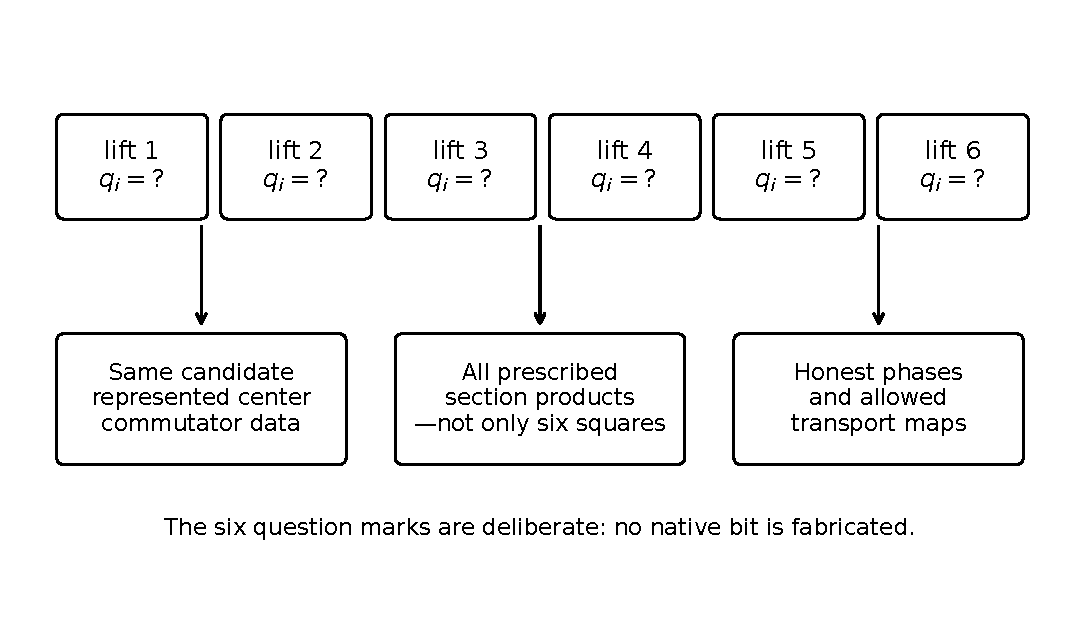
\includegraphics[width=\linewidth]{figures/V30.pdf}\end{center}
When the stronger contract independently fixes a native rank-eight marking, the certificate must name the actual candidate, the relevant finite subgroup and represented center, and the six genuine lifts of a symplectic basis. Their squares determine six bits only after those lifts and the two-element central representation have been established.
\[
q_W(v_i)\in\F_2\quad\text{must come from the actual lift square.}
\]
All prescribed section products must also be verified. Genuine extension actions do not by themselves choose the required honest representation phases. The certificate must state which maps or lifts may change and verify the resulting transport conditions.

No native square bit is supplied by this atlas. The data file records these fields as null, and the tests ensure they remain uncomputed rather than silently assigning zero. This is a conditional stronger obligation. It is not an extra premise inserted into the already valid transported-marking contract, where the finite marking is carried through the chosen comparison map.
\vfill\PlateSource{Unresolved arithmetic certificate}{Part III, Section 30.2}{75}
